\documentclass[conference]{IEEEtran}
\IEEEoverridecommandlockouts
% The preceding line is only needed to identify funding in the first footnote. If that is unneeded, please comment it out.
\usepackage{cite}
\usepackage{amsmath,amssymb,amsfonts}
\usepackage{algorithmic}
\usepackage{graphicx}
\usepackage{textcomp}
\usepackage{xcolor}

\usepackage[most]{tcolorbox}
\usepackage{multirow}

% \usepackage{graphicx}
% \usepackage{booktabs}
% \usepackage{amsmath,amssymb}
\usepackage{url}
% \usepackage{subcaption}
% \usepackage{float}

% preamble
\usepackage{tabularx}
\usepackage{booktabs}
\newcolumntype{W}{>{\hsize=1.25\hsize\raggedright\arraybackslash}X}
\newcolumntype{N}{>{\hsize=0.75\hsize\raggedright\arraybackslash}X}

\def\BibTeX{{\rm B\kern-.05em{\sc i\kern-.025em b}\kern-.08em
    T\kern-.1667em\lower.7ex\hbox{E}\kern-.125emX}}
\begin{document}

\title{GPU Adaptive Tracing\\
% {\footnotesize \textsuperscript{*}Note: Sub-titles are not captured in Xplore and
% should not be used}
% \thanks{Identify applicable funding agency here. If none, delete this.}
}

\author{\IEEEauthorblockN{1\textsuperscript{st} Sneh Patel}
\IEEEauthorblockA{\textit{dept. name of organization (of Aff.)} \\
\textit{name of organization (of Aff.)}\\
City, Country \\
email address or ORCID}
\and
\IEEEauthorblockN{2\textsuperscript{nd} Given Name Surname}
\IEEEauthorblockA{\textit{dept. name of organization (of Aff.)} \\
\textit{name of organization (of Aff.)}\\
City, Country \\
email address or ORCID}
\and
\IEEEauthorblockN{3\textsuperscript{rd} Given Name Surname}
\IEEEauthorblockA{\textit{dept. name of organization (of Aff.)} \\
\textit{name of organization (of Aff.)}\\
City, Country \\
email address or ORCID}
\and
}

\maketitle


\begin{abstract}
GPU profiling tools provide rich kernel-level evidence for diagnosing performance anomalies in LLM serving systems, but they are typically invoked manually with fixed profiling windows that neither adapt to evidence quality nor decide when enough has been collected. We present an \emph{adaptive GPU tracing controller} that manages heavy GPU profiling automatically using a two-tier evidence model: cheap always-on signals (request latency, throughput, GPU utilization, and GPU memory utilization) run continuously, while short Nsight Systems kernel-timing bursts are activated only when cheap evidence is insufficient to explain an anomaly and stopped as soon as the diagnosis has stabilized.

We design and evaluate six short-burst stopping policies, ranging from a single fixed burst to a hybrid policy that requires both diagnosis stability and workload recovery before de-escalating. Experiments on NVIDIA~L4 and A100~GPUs using vLLM serving \texttt{Qwen2.5-7B-Instruct} across six serving scenarios and three controlled microbenchmark workloads show that the adaptive controller reduces profiler duration by 18.9\%--48.5\% and captured kernel instances by 42.9\%--78.2\% relative to a manual fixed-window baseline, while preserving a top-1 diagnosis match rate of 1.0 across all workloads. Dedicated runtime-overhead measurements show that the cheap controller metrics introduce less than 1\% mean p95 latency regression on the serving workload. Policy comparison reveals that a single fixed burst fails under ambiguous first-window conditions, while the Hybrid Stop and Counter-Recovery Stop policies eliminate re-escalation at the cost of modest additional tracing. Signal analysis identifies diagnosis stability as the only stopping signal that consistently avoids firing on ambiguous windows across both stable and stress evaluation conditions.
\end{abstract}


\section{Introduction}

Large language model~(LLM) serving systems must sustain high throughput and predictable latency in production, yet they are routinely disrupted by performance anomalies: request queueing~\cite{yu2022orca}, compute saturation~\cite{agrawal2023sarathi}, memory pressure, long input or output sequences, or transient workload shifts. Diagnosing the root cause of such an anomaly often requires kernel-level evidence -- execution timing, launch frequency, duration distributions -- that only a GPU profiler such as NVIDIA Nsight Systems can provide; cheap runtime counters can reveal that something is wrong but rarely explain why. This kernel-level evidence is expensive to collect, so operators typically invoke the profiler manually with a fixed time window chosen by convention rather than by the state of the diagnosis.

This creates a tension between profiling cost and diagnostic confidence. A fixed-window profiler that runs too briefly may stop before the bottleneck class has stabilized into a concrete diagnosis, while one that runs too long wastes profiler time and storage recording redundant kernel evidence after the diagnosis has already converged. Existing practice offers no principled way to decide, while a profiling session is active, whether enough evidence has been collected to stop.

We address this gap with an \emph{adaptive GPU tracing controller} that automatically manages heavy GPU profiling for LLM serving systems, building on runtime-adaptive evidence escalation~\cite{mace2015pivot,zhang2023hindsight}. The controller organizes evidence into two tiers: cheap signals (request latency, throughput, GPU utilization, and GPU memory utilization) are collected continuously at negligible cost, while short Nsight Systems kernel-timing bursts are activated only when the cheap evidence is insufficient to explain an anomaly, and are stopped automatically once the kernel-level diagnosis has stabilized. Here, \emph{adaptive} describes the controller's escalation and de-escalation behavior, not a learned policy: the controller is a deterministic finite-state machine governed by fixed, hand-tuned thresholds (e.g., latency-regression ratio, GPU utilization, diagnosis-stability window count); no model is trained or fitted online. We design and evaluate six short-burst \emph{stopping policies} -- ranging from a single fixed burst to a hybrid policy that requires both diagnosis stability and workload recovery before de-escalating -- and identify which runtime signals most reliably indicate that sufficient evidence has been collected.

We evaluate the controller on NVIDIA L4 and A100 GPUs using vLLM serving \texttt{Qwen2.5-7B-Instruct} across six serving scenarios and three controlled microbenchmark workloads, guided by five research questions:

\begin{itemize}
  \item \textbf{RQ1:} Can the controller determine when sufficient diagnostic evidence has been collected, stopping heavy tracing earlier than a fixed-window baseline without sacrificing accuracy?
  \item \textbf{RQ2:} How accurate is automatic GPU tracing compared with manual fixed-window profiling?
  \item \textbf{RQ3:} Does automatic GPU tracing introduce measurable overhead compared with manual profiling?
  \item \textbf{RQ4:} Which short-burst GPU tracing stopping policies work best, and what tradeoffs do they make between cost and reliability?
  \item \textbf{RQ5:} Which runtime signals are most useful for deciding when to stop heavy GPU tracing?
\end{itemize}

\subsection{Contributions}

This paper makes the following contributions:

\begin{enumerate}
  \item A formulation of automatic GPU trace stopping as a runtime control problem, separate from anomaly detection and from the profiling mechanism itself.
  \item The design and implementation of a rule-based adaptive controller realizing this formulation as a working system: a finite-state machine driven by fixed, hand-tuned evidence thresholds (Table~\ref{tab:setup-params}) rather than a learned or online-trained policy.
  \item A comparative evaluation of six stopping policies along premature-stop rate and re-escalation rate, including a controlled ambiguity-stress condition that separates policies robust to an inconclusive first burst from those that are not.
  \item Evidence that automatic tracing matches manual fixed-window diagnosis accuracy while reducing profiler duration by 18.9\%--48.5\% and captured kernel instances by 42.9\%--78.2\%, with less than 1\% mean p95 latency overhead from the always-on cheap metrics.
  \item A signal-level analysis identifying diagnosis stability as the only stopping signal safe against ambiguous evidence, and characterizing why intuitive recovery-based signals are not.
\end{enumerate}
\section{Related Work}
\label{sec:related-work}

Work relevant to adaptive, budget-aware GPU tracing spans three bodies of literature: distributed tracing systems that decide what request-level evidence to collect, GPU profiling tools that expose accelerator-level evidence, and GPU-heavy LLM serving systems that produce the ambiguous bottlenecks our controller diagnoses.

\paragraph{Adaptive tracing.}
Production tracing systems such as Dapper~\cite{sigelman2010dapper}, X-Trace~\cite{fonseca2007xtrace}, and Canopy~\cite{kaldor2017canopy} established always-on, low-cost request-level tracing, but treat neither GPU execution nor kernel launches as first-class evidence. More recent systems move beyond fixed instrumentation toward runtime-adaptive collection: TraStrainer~\cite{huang2024trastrainer} combines trace diversity with system runtime state (CPU and memory pressure) to drive online sampling decisions, conceptually mirroring our use of GPU utilization and memory pressure as the cheap signal tier, while Astraea~\cite{toslali2024astraea} formalizes tracing as a cost-constrained online learning problem under a budget -- the closest existing budget formalism we build on. Neither, however, treats GPU profiler activation or kernel-level tracing as a tiered evidence source with its own escalation and de-escalation policy.

Both adapt a single scalar -- per-request sampling rate -- over distributed trace spans rather than activating a discrete GPU evidence tier, so we treat them as conceptually related rather than as ported baselines and leave a learned, budget-constrained GPU stopping policy as future work.

\paragraph{GPU profiling tools.}
NVBit~\cite{villa2019nvbit} provides dynamic binary instrumentation for fine-grained GPU kernel tracing, representative of the heaviest tier in our evidence hierarchy. HPCToolkit~\cite{zhou2021hpctoolkit} supports multiple evidence modes -- hardware counters, PC sampling, kernel tracing -- giving a practical existence proof of the multi-tier GPU evidence hierarchy our controller adopts. Both, however, assume a human operator or an offline workflow decides when to invoke the profiler and for how long; neither includes a runtime policy that activates, extends, or stops collection based on diagnostic sufficiency.

\paragraph{LLM serving systems.}
vLLM's PagedAttention~\cite{kwon2023vllm} demonstrates how GPU memory pressure, batching, and request latency interact during LLM serving, producing exactly the ambiguous, multi-cause bottlenecks that justify escalating to kernel-level evidence and that make premature de-escalation risky. We use vLLM as the concrete serving substrate on which our controller is evaluated.

Our work sits at the intersection of these three areas: it adopts the adaptive, budget-aware control philosophy of systems such as TraStrainer and Astraea, applies it to the GPU evidence sources exposed by tools such as NVBit and HPCToolkit, and evaluates it on the realistic, ambiguous bottlenecks produced by LLM serving systems such as vLLM. To our knowledge, no prior work studies the runtime control problem of automatically starting, continuing, and stopping costly GPU tracing while preserving diagnosis quality.


\section{Methodology}


\subsection{System Overview}

GPU-heavy serving systems such as large language model~(LLM) inference engines can experience performance anomalies for many reasons: request queueing, compute saturation, memory pressure, long input or output sequences, or transient workload shifts. Cheap always-on performance telemetry can reveal that something is wrong but often cannot explain why. Heavy GPU profiling can explain why, but it is expensive, typically invoked manually, and usually runs for a fixed window regardless of whether the collected evidence is already sufficient.

We present an \emph{adaptive GPU tracing controller} that bridges these two extremes. The controller collects cheap evidence continuously and activates a short burst of heavy GPU profiling only when cheap evidence is insufficient to explain an anomaly. After each burst it evaluates whether the collected kernel-level evidence has stabilized into a
diagnosis. When additional profiling would no longer change that diagnosis, the controller stops heavy tracing and returns to cheap-only monitoring.

\subsubsection{Evidence Tiers}

The controller organizes evidence into three tiers ordered by collection cost, summarized in Table~\ref{tab:evidence-tiers}.

\begin{table}[h]
\centering
\caption{Evidence tiers used by the adaptive tracing controller.}
\label{tab:evidence-tiers}
\scriptsize
\setlength{\tabcolsep}{4pt}
\renewcommand{\arraystretch}{1.2}
\begin{tabularx}{\columnwidth}{@{}l W N l@{}}
\toprule
\textbf{Tier} & \textbf{Signals} & \textbf{Collection mode} & \textbf{Cost} \\
\midrule
T0 & Request latency (p50, p95), throughput (req/s), queueing-delay proxy
   & Always-on, per request
   & Negligible \\
\addlinespace
T1 & GPU utilization, GPU memory utilization, SM clock, power draw
   & Always-on, NVML polling
   & Negligible \\
\addlinespace
T2 & Kernel execution timing, duration distribution, kernel launch frequency
   & Short profiler burst, Nsight Systems CLI
   & High \\
\bottomrule
\end{tabularx}
\end{table}

T0 and T1 signals are sampled continuously and aggregated into fixed-size time windows (10\,s in all experiments). T2 evidence is collected only when the controller determines that T0/T1 evidence alone is insufficient to identify the bottleneck class. T2 collection is bounded to a short burst duration and does not run continuously.

\subsubsection{Controller State Machine}

The controller operates as a finite-state loop over evidence windows. Figure~\ref{fig:state-machine} illustrates the five states and the transitions between them.

\begin{figure*}[t]
\centering
\begin{tikzpicture}[
  node distance=1.85cm,
  state/.style={draw, rounded corners, fill=gray!10, minimum width=1.9cm, minimum height=0.9cm, align=center, font=\small},
  >=Stealth, thick
]
\node[state] (idle) {Idle};
\node[state, right=of idle] (susp) {Suspicious};
\node[state, right=of susp] (trace) {Tracing};
\node[state, right=of trace] (eval) {Evaluating};
\node[state, right=of eval] (rec) {Recovered};

\draw[->] (idle) -- node[above, font=\scriptsize]{anomaly detected} (susp);
\draw[->] (susp) -- node[above, font=\scriptsize]{T2 triggered} (trace);
\draw[->] (trace) -- node[above, font=\scriptsize]{burst complete} (eval);
\draw[->] (eval) -- node[above, font=\scriptsize]{stop} (rec);
\draw[->] (eval) to[out=250,in=290,looseness=2.2] node[below=2pt, font=\scriptsize]{continue} (trace);
\draw[->] (rec) to[out=110,in=70,looseness=0.65] node[above=2pt, font=\scriptsize, align=center]{recovered: signals \& diagnosis\\stable $\geq 2$ windows; reset budget} (idle);
\end{tikzpicture}
\caption{Controller state machine. The controller escalates from \textsc{Idle} through \textsc{Suspicious} and \textsc{Tracing} to \textsc{Evaluating}, which either launches another burst (returning to \textsc{Tracing}) or de-escalates to \textsc{Recovered}; the controller returns to \textsc{Idle} once cheap signals and diagnosis stability both confirm recovery.}
\label{fig:state-machine}
\end{figure*}

In \textsc{Evaluating}, the controller classifies the bottleneck from the kernel summary (kernel count, total and mean kernel time, top kernel name) combined with the current T0/T1 window, then applies the active stopping policy to decide whether to stop or launch another burst.


\subsubsection{Windowing and Aggregation}

Evidence is aggregated over non-overlapping fixed-size time windows. Within each window the controller computes:

\begin{itemize}
  \raggedright
  \item \textbf{Latency statistics}: mean, p50, p95 request latency; ratio versus the initial-window baseline.
  \item \textbf{Throughput}: requests per second; ratio versus the initial-window baseline.
  \item \textbf{Queueing delay proxy}: difference between request completion time and a minimum expected service time, aggregated at p95 across the window.
  \item \textbf{GPU utilization}: mean and standard deviation of NVML \texttt{utilization.gpu} samples taken every 0.5\,s during the window.
  \item \textbf{GPU memory utilization}: mean NVML \texttt{utilization.memory} and used-memory fraction.
  \item \textbf{Diagnosis stability streak}: number of consecutive windows for which the top bottleneck class has remained unchanged.
  \item \textbf{Recovery streaks}: number of consecutive windows for which each recovery condition (latency, throughput, queueing delay, GPU utilization) has been satisfied.
\end{itemize}

When T2 evidence is available for a window, the controller additionally records the kernel summary extracted from the Nsight Systems report: total kernel instances, total kernel time, mean kernel duration, kernel duration coefficient of variation~(CV), and the name of the most time-consuming kernel.


\subsubsection{Anomaly Detection}

A window is marked suspicious when any of the following conditions holds:

\begin{enumerate}
  \item \textbf{Latency regression}: the current window p95 latency exceeds $1.5\times$ the initial-window p50 baseline.
  \item \textbf{High GPU utilization}: mean GPU utilization exceeds 85\% for two or more consecutive windows while request latency is also elevated.
  \item \textbf{High kernel launch rate}: the kernel launch frequency in the current window is more than $2\times$ the observed baseline, indicating many short-lived kernels.
\end{enumerate}

A suspicious window that already carries a stable bottleneck classification does not re-trigger T2 profiling. T2 is triggered only when the window is suspicious and the current diagnosis is absent, ambiguous, or unstable.

\subsubsection{Tracing Budget}

Each anomaly episode is capped at six profiler bursts. Budget exhaustion forces de-escalation and is logged as a distinct stop reason. In our experiments, the active stopping policy de-escalated before reaching this limit.


\subsection{Short-Burst Stopping Policies}
\label{sec:stopping-policies}
A stopping policy controls when the controller de-escalates from heavy GPU tracing back to cheap-only monitoring. After each profiler burst, the controller invokes the active policy to decide whether to launch another burst or stop. We define six candidate policies that span the spectrum from aggressive cost reduction to conservative reliability, applying the same cost-awareness behind adaptive and volume-reducing tracing decisions for distributed request traces~\cite{lascasas2019sifter,chen2024tracemesh,huang2024mint,chen2025tracezip,zhang2021threemilebeach} to GPU kernel-level evidence instead.


\subsubsection{Policy Definitions}

\paragraph{Fixed Burst (\textsc{FB}).}
Collect exactly one profiler burst after the first suspicious window, then stop. \textsc{FB} is the most aggressive fixed-count policy: it commits to a diagnosis from a single burst and never continues, making it the cheapest option but brittle when that one burst is ambiguous.

\paragraph{Repeated Fixed Burst (\textsc{RFB}).}
Collect a fixed number $N$ of bursts (default $N=3$), then stop regardless of diagnosis stability. \textsc{RFB} generalizes \textsc{FB} (which is the $N=1$ case): it buys more evidence than a single burst but, like \textsc{FB}, ignores whether that evidence has converged. It serves as the evidence-blind, fixed-cost baseline against which the adaptive policies (\textsc{SS}, \textsc{MU}) are compared.

\paragraph{Stability Stop (\textsc{SS}).}
Continue collecting bursts until the bottleneck class label has remained unchanged for $K$ consecutive evidence windows (default $K=2$), then stop. \textsc{SS} is evidence-aware: it collects more bursts when early windows are ambiguous and fewer when the label is clear from the start.

\paragraph{Marginal Utility Stop (\textsc{MU}).}
\textsc{MU} is the aggressive special case of \textsc{SS} with $K=1$: it stops as soon as one burst reproduces the previous burst's label, treating a single repeat as evidence that further bursts add no diagnostic value. Because it requires only one match rather than $K$ consecutive matches, it collects fewer bursts than \textsc{SS} but is more vulnerable to stopping on a transient agreement that later windows would contradict.

\paragraph{Counter-Recovery Stop (\textsc{CR}).}
Continue collecting bursts until T0/T1 cheap signals return to their pre-anomaly baselines: specifically, until p95 request latency drops below $1.1\times$ the initial-window baseline and GPU utilization drops below 60\%. If recovery does not occur before the budget is exhausted, the controller stops at budget. \textsc{CR} couples de-escalation to observable workload recovery rather than to diagnosis stability, making it robust against scenarios where the bottleneck clears before the diagnosis has converged.

\paragraph{Hybrid Stop (\textsc{HS}).}
Stop only when \emph{both} conditions hold: (1) the diagnosis has been stable for $K$ consecutive windows (as in \textsc{SS}), and (2) T0/T1 cheap signals show sustained recovery (as in \textsc{CR}). \textsc{HS} is the most conservative policy: it requires corroborating evidence from both the kernel-level diagnosis and the cheap runtime signals before committing to de-escalation. Neither condition alone is sufficient.

\subsubsection{Policy Summary}

Table~\ref{tab:policies} summarizes the six policies, their stopping conditions, and the primary tradeoff each makes between tracing cost and stopping reliability.

\begin{table*}
\centering
\caption{Short-burst stopping policies compared by stopping condition and cost--reliability tradeoff.}
\label{tab:policies}
\footnotesize
\setlength{\tabcolsep}{4pt}
\renewcommand{\arraystretch}{0.95}
\begin{tabularx}{\textwidth}{@{}l l >{\raggedright\arraybackslash}X >{\raggedright\arraybackslash}X@{}}
\toprule
\textbf{Policy} & \textbf{Abbrev.} & \textbf{Stopping condition} & \textbf{Primary tradeoff} \\
\midrule
Fixed Burst           & \textsc{FB}  & After 1 burst                                      & Cheapest; brittle on ambiguous first burst \\
Repeated Fixed Burst  & \textsc{RFB} & After $N$ bursts                                   & Predictable cost; ignores convergence \\
Stability Stop        & \textsc{SS}  & Bottleneck class stable for $K$ windows            & Evidence-aware; may over-collect on slow-stabilizing workloads \\
Marginal Utility Stop & \textsc{MU}  & New burst matches previous diagnosis               & Stops at first convergence; slightly more aggressive than \textsc{SS} \\
Counter-Recovery Stop & \textsc{CR}  & T0/T1 signals return to baseline                   & Workload-aware; may collect more when recovery is slow \\
Hybrid Stop           & \textsc{HS}  & Diagnosis stable \emph{and} T0/T1 signals recover  & Most conservative; lowest re-escalation risk \\
\bottomrule
\end{tabularx}
\end{table*}


% \subsubsection{Policy Parameters}

% All policies share a common parameter set that is held constant across experiments. Table~\ref{tab:policy-params} lists the values used in this paper.

% \begin{table}[h]
% \centering
% \caption{Policy parameter values used in all experiments.}
% \label{tab:policy-params}
% \begin{tabular}{lll}
% \toprule
% \textbf{Parameter} & \textbf{Value} & \textbf{Used by} \\
% \midrule
% Stability window count $K$           & 2     & \textsc{SS}, \textsc{HS} \\
% Repeated burst count $N$             & 3     & \textsc{RFB} \\
% Maximum budget (burst cap)           & 6     & All policies \\
% Latency recovery ratio               & 1.10  & \textsc{CR}, \textsc{HS} \\
% GPU utilization recovery threshold   & 60\%  & \textsc{CR}, \textsc{HS} \\
% \bottomrule
% \end{tabular}
% \end{table}

\subsubsection{Stopping Signals}

Each policy is implemented in terms of one or more \emph{stopping signals}: boolean or numeric per-window features that the controller evaluates after each burst. Table~\ref{tab:stopping-signals} lists the candidate signals studied in this paper. Section~\ref{sec:rq5} (RQ5) evaluates which signals are most reliable for predicting correct de-escalation points.

\begin{table}[h]
\centering
\caption{Candidate stopping signals evaluated in this paper.}
\label{tab:stopping-signals}
\scriptsize
\setlength{\tabcolsep}{3pt}
\begin{tabularx}{\columnwidth}{@{}l >{\raggedright\arraybackslash}X@{}}
\toprule
\textbf{Signal} & \textbf{Definition} \\
\midrule
\texttt{diagnosis\_stable\_2}            & Top bottleneck class unchanged for $\geq 2$ consecutive windows \\
\texttt{diagnosis\_changed\_from\_prev}  & Top bottleneck class differs from the immediately preceding window \\
\texttt{diagnosis\_margin\_clear}        & Confidence margin between top and runner-up diagnosis exceeds threshold \\
\texttt{latency\_recovered}              & p95 latency below $1.1\times$ initial-window baseline \\
\texttt{throughput\_recovered}           & Throughput above $0.9\times$ initial-window baseline \\
\texttt{queue\_delay\_recovered}         & p95 queueing delay proxy below recovery threshold \\
\texttt{gpu\_util\_recovered}            & Mean GPU utilization below 60\% \\
\texttt{memory\_pressure\_low}           & GPU memory used fraction below 80\% \\
\texttt{kernel\_duration\_stable}        & Kernel duration CV change across successive bursts below 10\% \\
\bottomrule
\end{tabularx}
\end{table}

% Diagnosis-evidence signals (\texttt{diagnosis\_stable\_2}, \texttt{diagnosis\_changed\_from\_prev}, \texttt{diagnosis\_margin\_clear}) depend only on the controller's kernel-summary classification  and are available whenever T2 evidence has been collected. Recovery signals (\texttt{latency\_recovered}, \texttt{throughput\_recovered}, \texttt{queue\_delay\_recovered}) depend on T0 request metrics and require a stable initial-window baseline. GPU counter signals (\texttt{gpu\_util\_recovered}, \texttt{memory\_pressure\_low}) depend on T1 NVML fields and are always available but may not vary meaningfully when the workload keeps the GPU consistently saturated. The kernel stability signal (\texttt{kernel\_duration\_stable}) requires at least two successive T2 bursts and is therefore unavailable to \textsc{FB}.


\subsection{Baselines}

We compare the adaptive controller against three baselines that model the range of existing profiling practices.


\paragraph{No Heavy Tracing (\textsc{NT}).}
The controller collects T0 and T1 evidence continuously but never activates a T2 profiler burst. Anomaly detection fires normally; the controller labels each suspicious window using cheap signals alone. \textsc{NT} represents the status quo for operators who rely entirely on utilization counters and request metrics for diagnosis, with no kernel-level profiling. It establishes the accuracy floor: any benefit from heavy tracing must exceed what T0/T1 evidence can provide on its own.

\paragraph{Manual Fixed-Window Profiling (\textsc{FW}).}
When an anomaly is detected, the controller starts a single Nsight Systems profiler burst of fixed duration, collects the kernel summary, produces a diagnosis, and stops. No further bursts are collected regardless of whether the diagnosis has stabilized. The fixed-window duration is set longer than the automatic burst duration to model a conservative manual profiling window (approximately $1.6\times$ to $2.0\times$ the automatic burst length across experiments).

\textsc{FW} models the standard operational practice of a developer or operator who: (1) notices an anomaly, (2) starts a profiler with a fixed rule such as ``profile for 30 seconds,'' (3) reads the resulting kernel report, and (4) stops. The fixed duration is chosen conservatively so that \textsc{FW} is not handicapped by an unrealistically short window; any savings from the adaptive controller are conservative estimates.

\paragraph{Always-Profile (\textsc{AP}).}
The T2 profiler remains active for the entire duration of the anomaly episode, from the first suspicious window until the controller observes sustained recovery. \textsc{AP} represents the upper bound on profiling cost: it collects the maximum possible kernel evidence but does not attempt to stop early. It is included to bound the overhead side of the comparison: if the adaptive controller approaches \textsc{AP} accuracy while using far less profiler time, the cost reduction is clearly worthwhile.

% \subsubsection{Baseline Summary}

% Table~\ref{tab:baselines} summarizes the three baselines alongside the adaptive controller.

% \begin{table}[h]
% \centering
% \caption{Comparison of the adaptive controller and the three baselines.}
% \label{tab:baselines}
% \scriptsize
% \setlength{\tabcolsep}{3pt}
% \renewcommand{\arraystretch}{1.1}
% \begin{tabularx}{\columnwidth}{@{}>{\raggedright\arraybackslash}p{1.9cm} l l l >{\raggedright\arraybackslash}X@{}}
% \toprule
% & \textbf{T0/T1} & \textbf{T2 act.} & \textbf{T2 stopped by} & \textbf{Role} \\
% \midrule
% No Heavy Tracing (\textsc{NT})    & Always & Never             & ---             & Accuracy floor \\
% Manual Fixed-Window (\textsc{FW}) & Always & First anomaly     & Fixed timer     & Operational baseline \\
% Always-Profile (\textsc{AP})      & Always & First anomaly     & Recovery only   & Cost upper bound \\
% Adaptive Controller               & Always & T1 ambiguous      & Stopping policy & Proposed system \\
% \bottomrule
% \end{tabularx}
% \end{table}

% The primary comparison throughout this paper is between the adaptive controller and \textsc{FW}, since \textsc{FW} most closely models current practice. \textsc{NT} and \textsc{AP} are used to bound the accuracy--cost space from below and above, respectively.

\subsection{Implementation}

\subsubsection{Serving Stack}
% Our method uses vLLM~\cite{kwon2023vllm} v0.10.2 as the LLM serving system. vLLM is a widely-used open-source inference engine that implements PagedAttention for efficient KV-cache management and exposes an OpenAI-compatible HTTP API. All experiments serve \texttt{Qwen/Qwen2.5-7B-Instruct}~\cite{qwen2025}, a 7-billion-parameter instruction-tuned model. This model fits within 24\,GB of GPU memory with full BFloat16 precision, making it compatible with the NVIDIA~L4 and A100 GPUs used in our evaluation. The vLLM server is started with default settings except for the KV-cache token budget, which vLLM allocates automatically based on available GPU memory. On the L4~24\,GB host, vLLM reports approximately 64,704 KV-cache tokens and a maximum concurrency of roughly $15.8\times$ for 4096-token requests at startup.
Our method uses vLLM~\cite{kwon2023vllm} v0.10.2 as the LLM serving system. vLLM is an open-source inference engine that implements PagedAttention for efficient KV-cache management and exposes an OpenAI-compatible HTTP API. All experiments serve \texttt{Qwen/Qwen2.5-7B-Instruct}~\cite{qwen2025}, a 7-billion-parameter instruction-tuned model. The model runs in full BFloat16 precision on the NVIDIA~L4 and A100 GPUs used in our evaluation. Unless otherwise stated, vLLM uses its default configuration and automatically allocates the KV cache from available GPU memory. On the 24\,GB L4 host, this configuration provides approximately 64,704 KV-cache tokens.



\subsubsection{Cheap Metric Collection (T0 and T1)}

T0 request metrics are collected by the load-generation client, which records per-request start/end timestamps, HTTP status, estimated prompt/output token counts, and scenario/seed labels. At the end of each evidence window the client aggregates per-request records into window-level statistics: p50 and p95 latency, throughput in requests per second, request success rate, queueing delay proxy at p95, and ratio fields versus the initial-window baseline.

T1 GPU metrics are collected by a background NVML polling thread running at 0.5\,s intervals using \texttt{nvidia-ml-py}. At window close, the thread aggregates all samples taken during the window into mean and standard deviation for GPU utilization, GPU memory utilization, used memory in MiB, SM clock speed, and GPU power draw.

\subsubsection{Heavy Metric Collection (T2)}

T2 evidence is collected using the Nsight Systems command-line interface (\texttt{nsys}~2024.6), the same class of low-overhead GPU kernel tracing studied by Darche and Dagenais~\cite{darche2024lowoverhead}. When the controller activates a burst, it launches a child process under \texttt{nsys profile}, bounded by the target workload duration rather than a wall-clock \texttt{duration} flag. This avoids the process-termination behaviour that caused CUDA kernel tables to be absent in reports when \texttt{nsys} was given an explicit duration limit on some GPU hosts. The resulting kernel summary feeds a bottleneck classification scheme in the spirit of top-down GPU performance analysis~\cite{zhou2020topdown,hao2023drgpu}.


After the burst completes, the controller runs \texttt{nsys stats report cuda\_gpu\_kern\_sum} on the resulting \texttt{.nsys-rep} file and parses the CUDA GPU kernel summary into the window record: distinct kernel type count, total kernel instances, total and mean kernel execution time, duration CV, and the name of the most time-consuming kernel.

% \subsubsection{Bottleneck Classification}

% The controller assigns each suspicious window a bottleneck class label from a fixed vocabulary. For microbenchmark workloads the labels are: \texttt{compute\_bound}, \texttt{launch\_overhead\_or\_small\_kernel}, \texttt{mixed}, and \texttt{latency\_regression\_unknown\_gpu\_cause}. For vLLM serving workloads the labels are: \texttt{vllm\_healthy},\texttt{vllm\_queue\_pressure}, \texttt{vllm\_long\_prompt}, \texttt{vllm\_long\_output}, \texttt{vllm\_compute\_saturation}, \texttt{vllm\_kv\_cache\_pressure}, and \texttt{vllm\_latency\_regression\_unknown\_gpu\_cause}.

% Classification combines T0/T1 threshold rules with T2 kernel-summary features when available. The rules are deterministic and hand-specified rather than learned. The \texttt{unknown\_gpu\_cause} label is emitted when the anomaly trigger fires but no concrete bottleneck class can be assigned; it counts as ambiguous in all accuracy evaluations.

% \subsubsection{Logging and Reproducibility}

% Every run writes two output artefacts per evidence window:

% \begin{enumerate}
%   \item A per-request CSV file containing the raw request records.
%   \item A per-window CSV file containing aggregated T0/T1 statistics, controller state fields,
%         diagnosis fields, profiler cost fields, and all stopping-signal values.
% \end{enumerate}

% Each experiment is parameterized by a random seed passed to the load generator and recorded in the run summary JSON. Where multiple repetitions are reported, each repetition uses a distinct seed drawn from a pre-specified list, and all repetitions are aggregated before computing means and confidence intervals. An experiment manifest JSON records the GPU name, driver version, PyTorch version, Nsight Systems version, and key command-line settings for each run to support independent reproduction.

\section{Evaluation}

We evaluate the adaptive tracing controller across five research questions. RQ1 asks whether the controller can determine when sufficient diagnostic evidence has been collected. RQ2 asks how accurate automatic tracing is compared with manual fixed-window profiling. RQ3 measures the overhead introduced by the controller. RQ4 compares the six short-burst stopping policies. RQ5 identifies which runtime signals are most useful for deciding when to stop heavy GPU tracing.


% \subsection{Experimental Setup}

% Experiments run on two single-GPU cloud platforms: an NVIDIA L4 (24\,GB, Ada Lovelace, \texttt{sm\_89}) as the primary platform for all research questions, and an NVIDIA A100 (40\,GB, Ampere, \texttt{sm\_80}) for cross-GPU validation in RQ1. All vLLM scenarios serve \texttt{Qwen/Qwen2.5-7B-Instruct} using vLLM v0.10.2 in BFloat16 precision. Controller and policy parameters are fixed across experiments as listed in Table~\ref{tab:setup-params}. Each workload uses five repetitions for microbenchmarks or three seeded repetitions for vLLM experiments, with results reported as means.

\subsection{Experimental Setup}

Experiments run on two single-GPU cloud platforms: an NVIDIA L4 (24,GB, Ada Lovelace, \texttt{sm\_89}) as the primary platform for all research questions, and an NVIDIA A100 (40,GB, Ampere, \texttt{sm\_80}) for cross-GPU validation in RQ1. All vLLM scenarios use vLLM v0.10.2~\cite{kwon2023vllm}, an open-source inference engine that implements PagedAttention for efficient KV-cache management and exposes an OpenAI-compatible HTTP API. The system serves \texttt{Qwen/Qwen2.5-7B-Instruct}~\cite{qwen2025}, a 7-billion-parameter instruction-tuned model, in BFloat16 precision.

Unless otherwise stated, vLLM uses its default configuration and automatically allocates the KV cache from available GPU memory. This provides approximately 64,704 KV-cache tokens on the 24,GB L4 host and 334,016 tokens on the 40,GB A100 host. CUDA graph capture remains enabled throughout the experiments. Although graph replay groups multiple kernel launches into a single CPU-side submission, Nsight Systems still records the individual GPU kernels within each replayed graph; consequently, T2 kernel-level evidence, including execution time, launch frequency, and duration distributions, is unaffected.

Controller and policy parameters are fixed across experiments as listed in Table~\ref{tab:setup-params}. Each workload uses five repetitions for microbenchmarks or three seeded repetitions for vLLM experiments, with results reported as means.

\subsubsection{Controller Parameters}

Table~\ref{tab:setup-params} lists the controller and policy parameters held constant across all experiments.

\begin{table}[h]
\centering
\caption{Controller and policy parameters used in all experiments.}
\label{tab:setup-params}
\footnotesize
\setlength{\tabcolsep}{4pt}
\begin{tabularx}{\columnwidth}{@{}l l >{\raggedright\arraybackslash}X@{}}
\toprule
\textbf{Parameter} & \textbf{Value} & \textbf{Notes} \\
\midrule
Evidence window size               & 10\,s              & All experiments \\
Automatic burst duration           & $\approx$10--12\,s & Bounded by target process duration \\
Fixed-window burst duration        & $\approx$17--24\,s & $1.6\times$--$2.0\times$ automatic \\
Stability window count $K$         & 2                  & \textsc{SS}, \textsc{HS} \\
Repeated burst count $N$           & 3                  & \textsc{RFB} \\
Maximum tracing budget             & 6 bursts/episode   & All policies \\
Latency recovery ratio             & 1.10               & \textsc{CR}, \textsc{HS} \\
GPU utilization recovery threshold & 60\%               & \textsc{CR}, \textsc{HS} \\
NVML polling interval              & 0.5\,s             & T1 collection \\
\bottomrule
\end{tabularx}
\end{table}


\subsubsection{Repetitions and Seeds}

Microbenchmark experiments use five independent repetitions per workload, while vLLM serving experiments use three seeded repetitions per scenario; all results report means across repetitions and, where relevant, 95\% confidence interval half-widths.



\subsection{RQ1: Can the Controller Determine When Sufficient Diagnostic Evidence Has Been Collected?}

\subsubsection{Metrics}

We evaluate evidence sufficiency using trace-time saved, expected-label match rate, and burst-count stability, measured as the standard deviation ($\sigma$) of profiler bursts across repetitions. Trace-time saved is the reduction in total profiler-active duration relative to the fixed-window baseline. An RQ1 result is considered successful when trace-time savings are at least 25%, the expected-label match rate is at least 0.95, and $\sigma \leq 0.25$.

\subsubsection{Microbenchmark Results}

Table~\ref{tab:rq1-micro} reports the RQ1 microbenchmark results for both the L4 and A100 platforms across five repetitions per workload.

\begin{table}[h]
\centering
\caption{RQ1 microbenchmark results: automatic vs.\ fixed-window profiler duration (mean over 5 repetitions). All rows pass the combined success criterion.}
\label{tab:rq1-micro}
\resizebox{\columnwidth}{!}{%
\begin{tabular}{llrrrrr}
\toprule
\textbf{GPU} & \textbf{Workload} & \textbf{Auto (s)} & \textbf{Fixed (s)} &
\textbf{Saved (\%)} & \textbf{Match rate} & \textbf{Burst $\sigma$} \\
\midrule
A100 & \texttt{compute\_bound}   & 10.4 & 16.7 & 37.6 & 1.0 & 0.0 \\
A100 & \texttt{launch\_overhead} & 11.9 & 23.2 & 48.5 & 1.0 & 0.0 \\
A100 & \texttt{mixed}            & 10.2 & 16.8 & 39.2 & 1.0 & 0.0 \\
\midrule
L4   & \texttt{compute\_bound}   & 12.4 & 18.1 & 31.6 & 1.0 & 0.0 \\
L4   & \texttt{launch\_overhead} & 13.0 & 24.0 & 45.8 & 1.0 & 0.0 \\
L4   & \texttt{mixed}            & 12.0 & 18.5 & 35.4 & 1.0 & 0.0 \\
\bottomrule
\end{tabular}%
}
\end{table}

The controller saves between 31.6\% and 48.5\% of profiler duration across all six workload-platform combinations while maintaining a perfect expected-label match rate of 1.0. Burst count standard deviation is 0.0 in every case: per-repetition logs show exactly one profiler burst in all 30 repetitions. This reflects the microbenchmark design, not insufficient variation between repetitions: each workload presents a single, unambiguous bottleneck signature from the first suspicious window, so diagnosis stability is already satisfied after one burst regardless of timing jitter. This single-burst convergence is specific to the controlled microbenchmarks; RQ2 and RQ4 (Section~\ref{sec:rq4}) show burst counts greater than one when the bottleneck class is less immediately separable. All rows pass the combined RQ1 success criterion.

Savings are consistently higher for \texttt{launch\_overhead\_or\_small\_kernel} than for \texttt{compute\_bound} or \texttt{mixed} on both GPUs. This is expected: the kernel summary for a high-launch-rate workload reveals its bottleneck class (many short kernels) after a short burst, allowing the stability condition to be satisfied quickly, whereas compute-bound and mixed workloads require a slightly longer burst to produce a stable GEMM-dominated summary.

Per-condition savings are stable: 95\% CI half-widths range from $\pm 0.5$ to $\pm 2.7$ points across the six combinations, an order of magnitude smaller than the 17-point spread between conditions.

% The A100 results are consistent in direction with the L4 results, with savings ranging from 37.6\% to 48.5\% on the A100 versus 31.6\% to 45.8\% on the L4. The modest difference in absolute savings is attributable to the A100's higher memory bandwidth and faster kernel execution times, which allow the diagnosis stability condition to be reached sooner within a burst.


\subsubsection{vLLM Serving Results}

On the \texttt{queue\_pressure} vLLM serving scenario, across three seeded repetitions on the L4, the controller reduces mean profiler duration from 133.5\,s (fixed-window) to 104.6\,s (automatic) -- a 21.7\% reduction (95\% CI $\pm 4.0$pp) -- while maintaining 100\% request success in every repetition.

\subsubsection{RQ1: Answer}

Yes. The adaptive controller determines when sufficient diagnostic evidence has been collected and stops heavy GPU tracing 21.7\%--48.5\% earlier than a manual fixed-window baseline across all evaluated workloads and GPU platforms, without sacrificing diagnosis accuracy.
\subsection{RQ2: How Accurate Is Automatic GPU Tracing Compared with Manual Profiling?}

\subsubsection{Metrics}

We evaluate diagnosis accuracy using expected-label match rate, ambiguous or unknown rate, time-to-diagnosis, and automatic-versus-fixed-window disagreement rate. Expected-label match rate is evaluated separately for automatic and fixed-window modes, with a success threshold of at least 0.95; the ambiguous or unknown rate has a target of at most 0.05. Time-to-diagnosis is the mean elapsed time from run start to the first window assigned the expected label. Disagreement measures the fraction of paired windows for which automatic and fixed-window modes assign different labels; disagreement alone is not an accuracy failure when both modes match the expected label in their respective suspicious windows.

\subsubsection{Microbenchmark Results}

Across all three L4 microbenchmark workloads and five repetitions each, automatic and fixed-window tracing achieved a 1.0 expected-label match rate and a 0.0 ambiguous rate. Both modes identified the expected bottleneck in the first evidence window, within approximately 5--6\,s.

\subsubsection{vLLM Multiclass Results}

Table~\ref{tab:rq2-vllm} reports RQ2 accuracy for the vLLM multiclass long-run experiments (three seeded repetitions per scenario, 402 per-window records total across six scenarios).

\begin{table*}[t]
\centering
\caption{RQ2 vLLM multiclass accuracy (3 seeds per scenario, L4). All six scenarios pass
all accuracy criteria in both modes. Auto trace and fixed-window trace columns report total
profiler duration across all repetitions.}
\label{tab:rq2-vllm}
\footnotesize
\setlength{\tabcolsep}{4pt}
\renewcommand{\arraystretch}{0.95}
\begin{tabular}{llrrrrrr}
\toprule
\textbf{Scenario} & \textbf{Mode} & \textbf{Match} & \textbf{Ambig.} &
\textbf{TTD (s)} & \textbf{Disagree} & \textbf{Trace (s)} & \textbf{Kernels} \\
\midrule
\texttt{healthy}
  & Auto  & 1.0 & 0.0 & 10.0 & \multirow{2}{*}{0.00} & 301.3 & 730K \\
  & Fixed & 1.0 & 0.0 & 10.0 &                        & 391.9 & 1380K \\
\midrule
\texttt{queue\_pressure}
  & Auto  & 1.0 & 0.0 & 10.0 & \multirow{2}{*}{0.00} & 309.7 & 748K \\
  & Fixed & 1.0 & 0.0 & 10.0 &                        & 403.4 & 1380K \\
\midrule
\texttt{long\_prompt}
  & Auto  & 1.0 & 0.0 & 10.0 & \multirow{2}{*}{0.25} & 290.4 & 732K \\
  & Fixed & 1.0 & 0.0 & 10.0 &                        & 381.0 & 1380K \\
\midrule
\texttt{long\_output}
  & Auto  & 1.0 & 0.0 & 10.0 & \multirow{2}{*}{0.00} & 291.0 & 729K \\
  & Fixed & 1.0 & 0.0 & 10.0 &                        & 397.1 & 1380K \\
\midrule
\texttt{compute\_saturation}
  & Auto  & 1.0 & 0.0 & 10.0 & \multirow{2}{*}{0.00} & 336.8 & 757K \\
  & Fixed & 1.0 & 0.0 & 10.0 &                        & 415.1 & 1380K \\
\midrule
\texttt{kv\_cache\_pressure}
  & Auto  & 1.0 & 0.0 & 10.0 & \multirow{2}{*}{0.00} & 329.4 & 731K \\
  & Fixed & 1.0 & 0.0 & 10.0 &                        & 449.3 & 1380K \\
\bottomrule
\end{tabular}
\end{table*}

% All six vLLM serving scenarios pass all accuracy criteria in both automatic and fixed-window modes. The expected-label match rate is 1.0, the ambiguous rate is 0.0, and time-to-diagnosis is the first 10\,s evidence window for every scenario and mode.
Automatic and fixed-window tracing satisfy all accuracy criteria across the six vLLM serving scenarios (Table~\ref{tab:rq2-vllm}), with a perfect expected-label match rate, zero ambiguous rate, and diagnosis in the first 10\,s evidence window.

% The disagreement rate is 0.0 for five of the six scenarios. The non-zero disagreement for \texttt{long\_prompt} (0.25) is again a sequence-level difference rather than an accuracy failure: both modes match the expected label on their respective suspicious windows.
Non-zero disagreement rates reflect sequence-level differences rather than diagnosis failures. \texttt{long\_prompt} is the only vLLM scenario with non-zero disagreement (0.25), because automatic mode stops collecting bursts earlier, so automatic and fixed-window tracing do not always assign profiler-enriched labels to the same windows; both modes still assign the correct expected label on every suspicious window.


% Across all six vLLM scenarios, automatic mode uses 1,858\,s of total profiler time against 2,438\,s for fixed-window mode, capturing 1,460K kernel instances against 2,759K for fixed-window mode. Automatic mode achieves the same accuracy while profiling for 23.8\% less time and recording 47.1\% fewer kernel instances.

Across all six vLLM scenarios, automatic mode achieves the same diagnosis accuracy as fixed-window tracing while profiling for 23.8\% less time and recording 47.1\% fewer kernel instances.


\subsubsection{RQ2: Answer}

Automatic GPU tracing matches the diagnosis accuracy of manual fixed-window profiling exactly: an expected-label match rate of 1.0 and an ambiguous rate of 0.0 across all microbenchmark workloads and all six vLLM serving scenarios, with time-to-diagnosis at the first evidence window in every case. Automatic mode reaches this accuracy using 23.8\% less profiler time and recording 47.1\% fewer kernel instances.

\subsection{RQ3: Does Automatic GPU Tracing Introduce Overhead Compared with Manual Profiling?}

We study overhead from two complementary angles. The first is \emph{profiler-cost overhead}: how much profiler time and how many profiled kernel instances does automatic tracing use compared with fixed-window profiling? The second is \emph{runtime perturbation}: does running the cheap controller metrics alongside vLLM introduce measurable degradation in request latency or throughput?

\subsubsection{Metrics}

\begin{itemize}
  \item \textbf{Trace-time saved (\%) and kernel instances avoided (\%).}
    Reduction in profiler-active duration and in the number of kernel instances recorded by the profiler, relative to the fixed-window baseline.
  \item \textbf{p95 latency regression (\%).}
    Change in p95 request latency between cheap-metrics mode and no-profiler mode, computed as $(p95_{\text{cheap}} - p95_{\text{none}}) / p95_{\text{none}} \times 100$. Positive values indicate regression; negative values indicate improvement.
  \item \textbf{Throughput change (\%).}
    Change in requests per second between cheap-metrics mode and no-profiler mode.
  \item \textbf{Request success rate.}
    Fraction of requests that completed successfully. Must remain at 100\%.
\end{itemize}

The RQ3 success criteria are: positive trace-time savings, positive kernel-instance reduction, p95 latency regression $\leq 5\%$, and request success rate of 100\%.

\subsubsection{Profiler-Cost Overhead}

Combining the RQ1 and RQ2 artifacts (Tables~\ref{tab:rq1-micro}--\ref{tab:rq2-vllm}), automatic tracing reduces profiler duration by 18.9\%--48.5\% and captured kernel instances by 42.9\%--78.2\% across all workloads, relative to the fixed-window baseline and while preserving a diagnosis match rate of 1.0. Microbenchmark workloads show higher savings than vLLM scenarios because their bottleneck classes stabilize more quickly.

\subsubsection{Dedicated Runtime Perturbation}

To isolate the cost of the cheap controller metrics, we compare a \emph{no-profiler} baseline against a \emph{cheap-metrics-only} mode (NVML polling and windowed metric aggregation, no Nsight profiling), randomizing which mode runs first in each repetition to control for run-order effects, across five randomized repetitions of \texttt{queue\_pressure} and three of \texttt{healthy}. All rows pass the RQ3 criteria.

The cheap controller metrics introduce no measurable p95 latency regression on either scenario. For \texttt{queue\_pressure} the mean p95 latency is 3.6\% \emph{lower} in cheap-metrics mode (5 reps, 95\% CI $\pm 6.3$ points), and for \texttt{healthy} the regression is $+0.6\%$ (3 reps, 95\% CI $\pm 1.9$ points), well within the 5\% threshold. Both intervals are wide given the small repetition counts, but even \texttt{queue\_pressure}'s upper bound ($+2.7\%$) clears the threshold with margin. Request success remains at 100\% in both scenarios and both modes.

Throughput change is small ($-0.5\%$ to $-1.0\%$) but more sensitive to run order than p95 latency; we report it as context rather than as a hard criterion.

\subsubsection{RQ3: Answer}

Automatic tracing reduces profiler cost substantially relative to fixed-window profiling without degrading serving performance: profiler duration drops by 18.9\%--48.5\% and captured kernel instances by 42.9\%--78.2\%. The cheap controller metrics introduce less than 1\% mean p95 latency change in the serving workload in five randomized repetitions, confirming that the controller overhead is negligible.


\subsection{RQ4: Which Short-Burst GPU Tracing Policies Work Best?}
\label{sec:rq4}

\subsubsection{Evaluation Approach}

RQ4 compares the six stopping policies via offline replay over real L4 vLLM window evidence, avoiding additional expensive Nsight executions per policy. Each policy is replayed over the same per-window evidence streams, so differences in outcome are attributable solely to the stopping condition rather than to workload variation or profiler noise. This assumes a policy's stopping choice does not meaningfully change later windows' evidence; we expect this confound to be small since T0/T1 collection is always-on and policy-independent, and RQ3 bounds the profiler's own T0/T1 perturbation at under 1\%.

We use two replay datasets. The \emph{stable replay} uses the real automatic-mode windows from the six vLLM serving scenarios across three seeds (18 streams). In this dataset the correct bottleneck label appears in the first suspicious window for every stream, making it an easy diagnostic setting. The \emph{ambiguity stress replay} uses the same 18 streams with the first suspicious window in each stream relabeled as unknown, modeling the realistic case where a single burst is insufficient. The stress dataset is the primary discriminating evaluation because it separates policies that can handle ambiguous early windows from those
that cannot.

\subsubsection{Metrics}

We report mean top-1 accuracy, premature-stop rate, re-escalation-needed rate (the fraction of streams with suspicious windows remaining after the policy stops), mean heavy-trace duration, and duration saved relative to the Repeated Fixed Burst baseline ($N=3$). These are combined into a composite score weighted 40\% accuracy, 25\% premature-stop avoidance, 20\% re-escalation avoidance, and 15\% cost-efficiency.\footnote{Composite score $= 0.40 \times \text{accuracy} + 0.25 \times (1 - \text{premature-stop rate}) + 0.20 \times (1 - \text{re-escalation rate}) + 0.15 \times \text{cost-efficiency}$, where cost-efficiency is the normalised inverse of mean trace duration.}

\subsubsection{Stable Replay Results}

The stable replay is not the discriminating condition --- every policy reaches top-1 accuracy of 1.0 with zero premature stops --- so its results are summarized in text rather than a table. \textsc{CR} and \textsc{HS} avoided re-escalation entirely but required 34.9\,s of tracing per episode, whereas \textsc{FB} used 10.0\,s but left suspicious windows after stopping. \textsc{MU} and \textsc{SS} were Pareto-dominated by \textsc{FB}: they incurred twice the tracing cost (20.0\,s) without improving accuracy or re-escalation rate. \textsc{RFB} fell between these extremes (30.0\,s, re-escalation rate 0.8) and remained Pareto-efficient only because no other policy matched its particular cost--reliability point.

\subsubsection{Ambiguity Stress Replay Results}

Table~\ref{tab:rq4-stress} reports policy rankings on the ambiguity stress dataset, which
is the primary discriminating evaluation.

\begin{table*}[t]
\centering
\caption{RQ4 ambiguity stress policy ranking (18 streams, first window relabeled as
unknown). \textsc{FB} fails entirely; multi-window policies recover to top-1 accuracy
of 1.0.}
\label{tab:rq4-stress}
\footnotesize
\setlength{\tabcolsep}{4pt}
\renewcommand{\arraystretch}{0.95}
\begin{tabular}{clrrrrrrl}
\toprule
\textbf{Rank} & \textbf{Policy} & \textbf{Top-1} & \textbf{Premature} &
\textbf{Re-esc.} & \textbf{Trace (s)} & \textbf{Saved (\%)} &
\textbf{Score} & \textbf{Pareto} \\
\midrule
1 & \textsc{CR} & 1.0 & 0.0 & 0.0 & 34.9 & $-16.3$ & 0.868 & yes \\
2 & \textsc{HS} & 1.0 & 0.0 & 0.0 & 34.9 & $-16.3$ & 0.868 & yes \\
3 & \textsc{MU} & 1.0 & 0.0 & 0.8 & 30.0 &    0.0  & 0.720 & yes \\
4 & \textsc{RFB} & 1.0 & 0.0 & 0.8 & 30.0 &   0.0  & 0.720 & yes \\
5 & \textsc{SS} & 1.0 & 0.0 & 0.8 & 30.0 &    0.0  & 0.720 & yes \\
6 & \textsc{FB} & 0.0 & 1.0 & 1.0 & 10.0 & $+66.7$ & 0.112 & yes \\
\bottomrule
\end{tabular}
\end{table*}

The stress dataset clearly separates one-burst and multi-burst policies.
\textsc{FB} fails completely: its top-1 accuracy drops to 0.0 and its premature-stop rate
rises to 1.0, because it commits to the ambiguous first-window unknown label and never
collects the additional burst needed to reach the concrete diagnosis.
Despite this failure, \textsc{FB} still shows Pareto-efficient in Table~\ref{tab:rq4-stress}, since no policy beats it on cost alone; Pareto status must therefore be read alongside accuracy and premature-stop rate, not as a standalone selection criterion.

All five multi-window policies recover to a top-1 accuracy of 1.0 and a premature-stop
rate of 0.0.
\textsc{CR} and \textsc{HS} again rank highest with a re-escalation rate of 0.0,
confirming their robustness as safety-first policies: they wait for both diagnosis
stability and workload recovery before stopping, ensuring no suspicious windows remain.

\textsc{MU}, \textsc{SS}, and \textsc{RFB} are tied at rank 3--5 with a re-escalation
rate of 0.83 and a mean trace duration of 30\,s. \textsc{MU} and \textsc{SS} are
preferable to \textsc{RFB} since they stop on evidence convergence rather than a
fixed burst count.

\subsubsection{Policy Tradeoff Analysis}

Figure~\ref{fig:rq4-tradeoff} illustrates the cost--safety tradeoff across the six
policies on the stress dataset.

\begin{figure}[t]
\centering
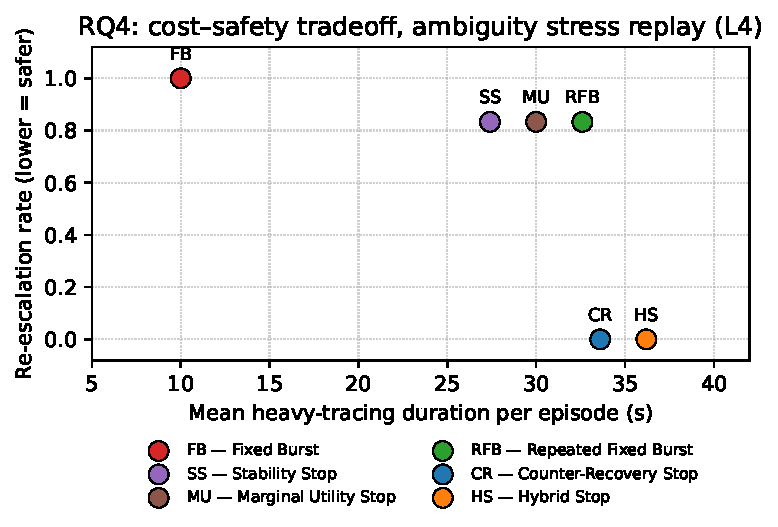
\includegraphics[width=\columnwidth]{figures/rq4_tradeoff.pdf}
\caption{Cost--safety tradeoff across the six stopping policies on the ambiguity stress dataset (Table~\ref{tab:rq4-stress}). \textsc{CR} and \textsc{HS} achieve zero re-escalation at higher trace cost; \textsc{MU}, \textsc{RFB}, and \textsc{SS} trade a 0.8 re-escalation rate for lower cost; \textsc{FB} is cheapest but fails outright (top-1 accuracy 0.0) rather than merely re-escalating.}
\label{fig:rq4-tradeoff}
\end{figure}

\subsubsection{RQ4: Answer}

No single policy dominates all dimensions, so the right choice depends on operator priorities. For safety-first deployments, \textsc{Hybrid Stop} and \textsc{Counter-Recovery Stop} eliminate re-escalation entirely and are robust to ambiguous first windows, at the cost of about 16\% more trace budget than \textsc{RFB}. For budget-aware deployments, \textsc{Stability Stop} and \textsc{Marginal Utility Stop} achieve 1.0 top-1 accuracy with 33\% less trace time than the recovery-gated policies, accepting a re-escalation rate of approximately 0.83. \textsc{Fixed Burst} is not robust as a standalone policy: it fails completely when the first profiler window is ambiguous, with a top-1 accuracy of 0.0 and a premature-stop rate of 1.0 on the stress dataset.
\subsection{RQ5: Which Runtime Signals Are Most Useful for Deciding When to Stop Heavy GPU Tracing?}
\label{sec:rq5}

\subsubsection{Evaluation Approach}

RQ5 evaluates the nine candidate stopping signals defined in Section~\ref{sec:stopping-policies} on two datasets.

\begin{itemize}
  \item[] \textbf{Real enriched L4 runs.} 18 vLLM serving runs (6 scenarios $\times$ 3 seeds, 60\,s per run) collected with the enriched window schema that includes non-sparse baseline ratio fields, recovery streak counters, and diagnosis confidence and margin fields. These runs provide a realistic serving signal distribution for evaluating which signals identify correct stopping points.
  \item[] \textbf{Ambiguity stress replay.} The same stress dataset used in RQ4 (first suspicious window relabeled as unknown). This dataset tests whether a signal fires on ambiguous stopping points as well as correct ones; a signal that cannot distinguish between the two is not safe to use as a standalone stopping criterion.
\end{itemize}

A signal is considered \emph{paper-ready} if it satisfies all three of the following criteria simultaneously: (1) precision $\geq 0.90$ on both datasets, (2) correct-stop F1 $\geq 0.70$ on the stress replay, and (3) ambiguous-stop F1 $\leq 0.10$ on the stress replay. Criterion (3) is the strictest filter: a signal that fires reliably on correct windows but also fires on ambiguous windows would cause the controller to stop too early when the diagnosis has not yet converged.

\subsubsection{Signal Ranking Results}

Table~\ref{tab:rq5-signals} reports precision, recall, and F1 for each candidate signal across the two evaluation datasets, together with the paper-ready verdict.

\begin{table*}[t]
\centering
\caption{RQ5 stopping signal ranking. Signals are sorted by composite score. Only
\texttt{diagnosis\_stable\_2} passes all paper-ready criteria.}
\label{tab:rq5-signals}
\footnotesize
\setlength{\tabcolsep}{4pt}
\renewcommand{\arraystretch}{0.95}
\begin{tabular}{lrrrrrrl}
\toprule
& \multicolumn{3}{c}{\textbf{Real enriched}} &
  \multicolumn{3}{c}{\textbf{Stress replay}} & \\
\cmidrule(lr){2-4} \cmidrule(lr){5-7}
\textbf{Signal} & \textbf{Prec.} & \textbf{Rec.} & \textbf{F1} &
\textbf{Prec.} & \textbf{F1 (correct)} & \textbf{F1 (ambig.)} &
\textbf{Paper-ready} \\
\midrule
\texttt{diagnosis\_stable\_2}   & 1.000 & 0.860 & 0.925 & 1.000 & 0.786 & 0.000 & \textbf{yes} \\
\texttt{latency\_recovered}     & 1.000 & 1.000 & 1.000 & 0.739 & 0.850 & 0.414 & no \\
\texttt{throughput\_recovered}  & 1.000 & 0.884 & 0.938 & 0.778 & 0.800 & 0.333 & no \\
\texttt{queue\_delay\_recovered}& 1.000 & 0.659 & 0.794 & 0.739 & 0.850 & 0.414 & no \\
\texttt{diagnosis\_margin\_clear}& 1.000 & 0.744 & 0.853 & 0.000 & 0.000 & 0.000 & no \\
\texttt{diagnosis\_changed}     & 1.000 & 0.465 & 0.635 & 1.000 & 0.522 & 0.000 & no \\
\texttt{gpu\_util\_recovered}   & 0.000 & 0.000 & 0.000 & 0.000 & 0.000 & 0.000 & no \\
\texttt{memory\_pressure\_low}  & 0.000 & 0.000 & 0.000 & 0.000 & 0.000 & 0.000 & no \\
\texttt{kernel\_duration\_stable}& 0.000 & 0.000 & 0.000 & 0.000 & 0.000 & 0.000 & no \\
\bottomrule
\end{tabular}
\end{table*}

\texttt{diagnosis\_stable\_2} is the only signal passing all three paper-ready criteria (Table~\ref{tab:rq5-signals}).

\subsubsection{Analysis of Individual Signal Groups}

\paragraph{Diagnosis-evidence signals.}
\texttt{diagnosis\_stable\_2} is the strongest and most defensible signal because it is derived directly from the kernel-level evidence the controller has already collected. It requires no external baseline calibration and does not depend on the workload's utilization or request rate returning to a specific threshold. Its main limitation is recall: on the real enriched runs it fires on 86\% of correct stopping points rather than all of them, meaning it occasionally requires one additional window before triggering.
\texttt{diagnosis\_margin\_clear} is promising on the real enriched runs (F1 0.853) but scores 0.000 on the stress replay, because the stress dataset predates the enriched schema and the margin field is absent.

\texttt{diagnosis\_changed} has perfect precision but low recall (F1 0.635 on real enriched runs). It is better understood as a \emph{continuation signal} than a stopping signal: when the diagnosis changes from one window to the next, the controller should continue tracing rather than stop. This is the inverse of its intended stopping role.

\paragraph{Recovery signals.}
\texttt{latency\_recovered} and \texttt{queue\_delay\_recovered} achieve the highest F1scores on the real enriched runs (1.000 and 0.794 respectively) but fail the paper-ready ambiguous-stop criterion with stress replay F1 values of 0.414. These signals fire on ambiguous stress windows because the stress transformation only relabels the diagnosis field, not the request latency values---latency recovery can therefore be observed even when the diagnosis is still unknown. They are valuable as supporting signals within the \textsc{CR} and \textsc{HS} policies, but they are not safe as standalone stopping signals.

\texttt{throughput\_recovered} shows a similar pattern: high F1 on real enriched runs (0.938) but fails the ambiguity criterion (stress F1 0.333).

\paragraph{GPU counter signals.}
At default thresholds (60\% util, 95\% memory), both score 0.000 since utilization never drops that low (observed range: 92.4--99.4\% util, 96.7--97.7\% memory). Recalibrating util to 99\% raises \texttt{gpu\_util\_recovered}'s recall to 0.953, but it then fires on 100\% of ambiguous windows (F1 0.419), violating the safety criterion; \texttt{memory\_pressure\_low} stays near-uninformative (recall 0.054) even at 97.5\%.

\paragraph{Kernel duration stability.}
\texttt{kernel\_duration\_stable} scores 0.000 because it requires two successive T2 bursts, and the \textsc{FB} policy used as the comparison baseline never collects a second burst.

\subsubsection{RQ5: Answer}

Diagnosis stability is the only stopping signal that is simultaneously precise, informative, and safe against ambiguous early windows. \texttt{diagnosis\_stable\_2} is the sole signal that passes all paper-ready criteria: it achieves 1.000 precision and an F1 of 0.925 on real enriched L4 runs, and never fires on ambiguous stopping points (stress ambiguous-stop F1 of 0.000). Recovery signals (\texttt{latency\_recovered}, \texttt{throughput\_recovered}) are strong on non-ambiguous workloads but fail the ambiguity safety criterion, making them suitable as supporting signals within \textsc{HS} and \textsc{CR} but not as standalone stopping criteria. GPU counter signals (\texttt{gpu\_util\_recovered}, \texttt{memory\_pressure\_low}) are inoperative for saturated LLM inference workloads.


\section{Threats to Validity}
\label{sec:threats}

Several factors limit the generalizability of these results. Internally, RQ4 and RQ5 rely on offline policy replay with a synthetic ambiguity injection manually relabeling the first suspicious window as unknown rather than naturally occurring ambiguous windows, and the bottleneck classification used to compute ground-truth labels is itself rule-based rather than independently verified. Externally, all experiments use a single model (\texttt{Qwen2.5-7B-Instruct}), a single serving framework (vLLM), a single profiler (Nsight Systems), and two GPU platforms (L4, A100); results may not transfer to other model architectures, serving stacks, or GPU generations. The finding that GPU-counter signals (\texttt{gpu\_util\_recovered}, \texttt{memory\_pressure\_low}) are inoperative is specific to saturated, high-concurrency serving and may not hold under lighter load, where utilization is more likely to dip below the recovery threshold. The RQ4 composite score uses a fixed weighting (40\% accuracy, 25\% premature-stop avoidance, 20\% re-escalation avoidance, 15\% cost-efficiency) that is a judgment call rather than an empirically derived tradeoff, and a different weighting could reorder policy rankings. Finally, repetition counts are modest (five microbenchmark repetitions, three vLLM seeds, eighteen replay streams), which limits the statistical power of the reported confidence intervals.

\section{Conclusion}

This paper presented an adaptive GPU tracing controller that resolves the tension between profiling cost and diagnostic confidence in LLM serving systems by collecting cheap evidence continuously and activating short, bounded Nsight Systems bursts only when needed, stopping as soon as the kernel-level diagnosis has stabilized. Across NVIDIA L4 and A100 GPUs, six vLLM serving scenarios, and three microbenchmark workloads, the controller reduced profiler duration by 18.9\%--48.5\% and captured kernel instances by 42.9\%--78.2\% relative to manual fixed-window profiling, while preserving a diagnosis match rate of 1.0 and introducing less than 1\% mean p95 latency overhead. Among the six stopping policies evaluated, Hybrid Stop and Counter-Recovery Stop eliminate re-escalation risk at modest additional cost, Stability Stop and Marginal Utility Stop offer a cheaper evidence-driven alternative, and a single Fixed Burst is unsafe under ambiguous first-window conditions; of the nine candidate stopping signals, only diagnosis stability reliably avoids firing on unconverged diagnoses. Together these results show that adaptive, evidence-driven control of heavy GPU profiling can substantially reduce tracing cost without sacrificing diagnostic accuracy, offering a practical alternative to today's all-or-nothing approach to GPU profiling in production LLM serving.

\clearpage
\label{page:lastmain}
\bibliographystyle{splncs04}
\bibliography{references}
\end{document}
